\subsection{Evaluation Design}

The evaluation strategy combined model metrics, software testing, and operational inspection. For machine learning metrics, fixed train-validation-test splits were used so that the final test set remained isolated from checkpoint selection. For software quality, automated tests covered API behaviour, preprocessing, routing, entity detection, model advisory, inference rules, and split utilities. For operational quality, the admin console and trace tools were used to inspect model behaviour under realistic phrases.

This multi-layer evaluation approach was necessary because the project was hybrid. A high intent accuracy alone would not have proved that final answers were appropriate, nor would a working UI alone have proved that the classifiers were reliable. The evaluation therefore examined the full path from phrase input to logged output.

\begin{table}[H]
    \centering
    \caption{Final held-out test metrics for the two model profiles.}
    \label{tab:final-metrics}
    \begin{tabular}{lccccc}
        \hline
        Model & Accuracy & Macro F1 & Weighted F1 & Macro Precision & Macro Recall \\
        \hline
        General & 0.8928 & 0.8649 & 0.8914 & 0.8822 & 0.8617 \\
        Report & 0.9358 & 0.8965 & 0.9360 & 0.8968 & 0.9040 \\
        \hline
    \end{tabular}
\end{table}

\begin{figure}[H]
    \centering
    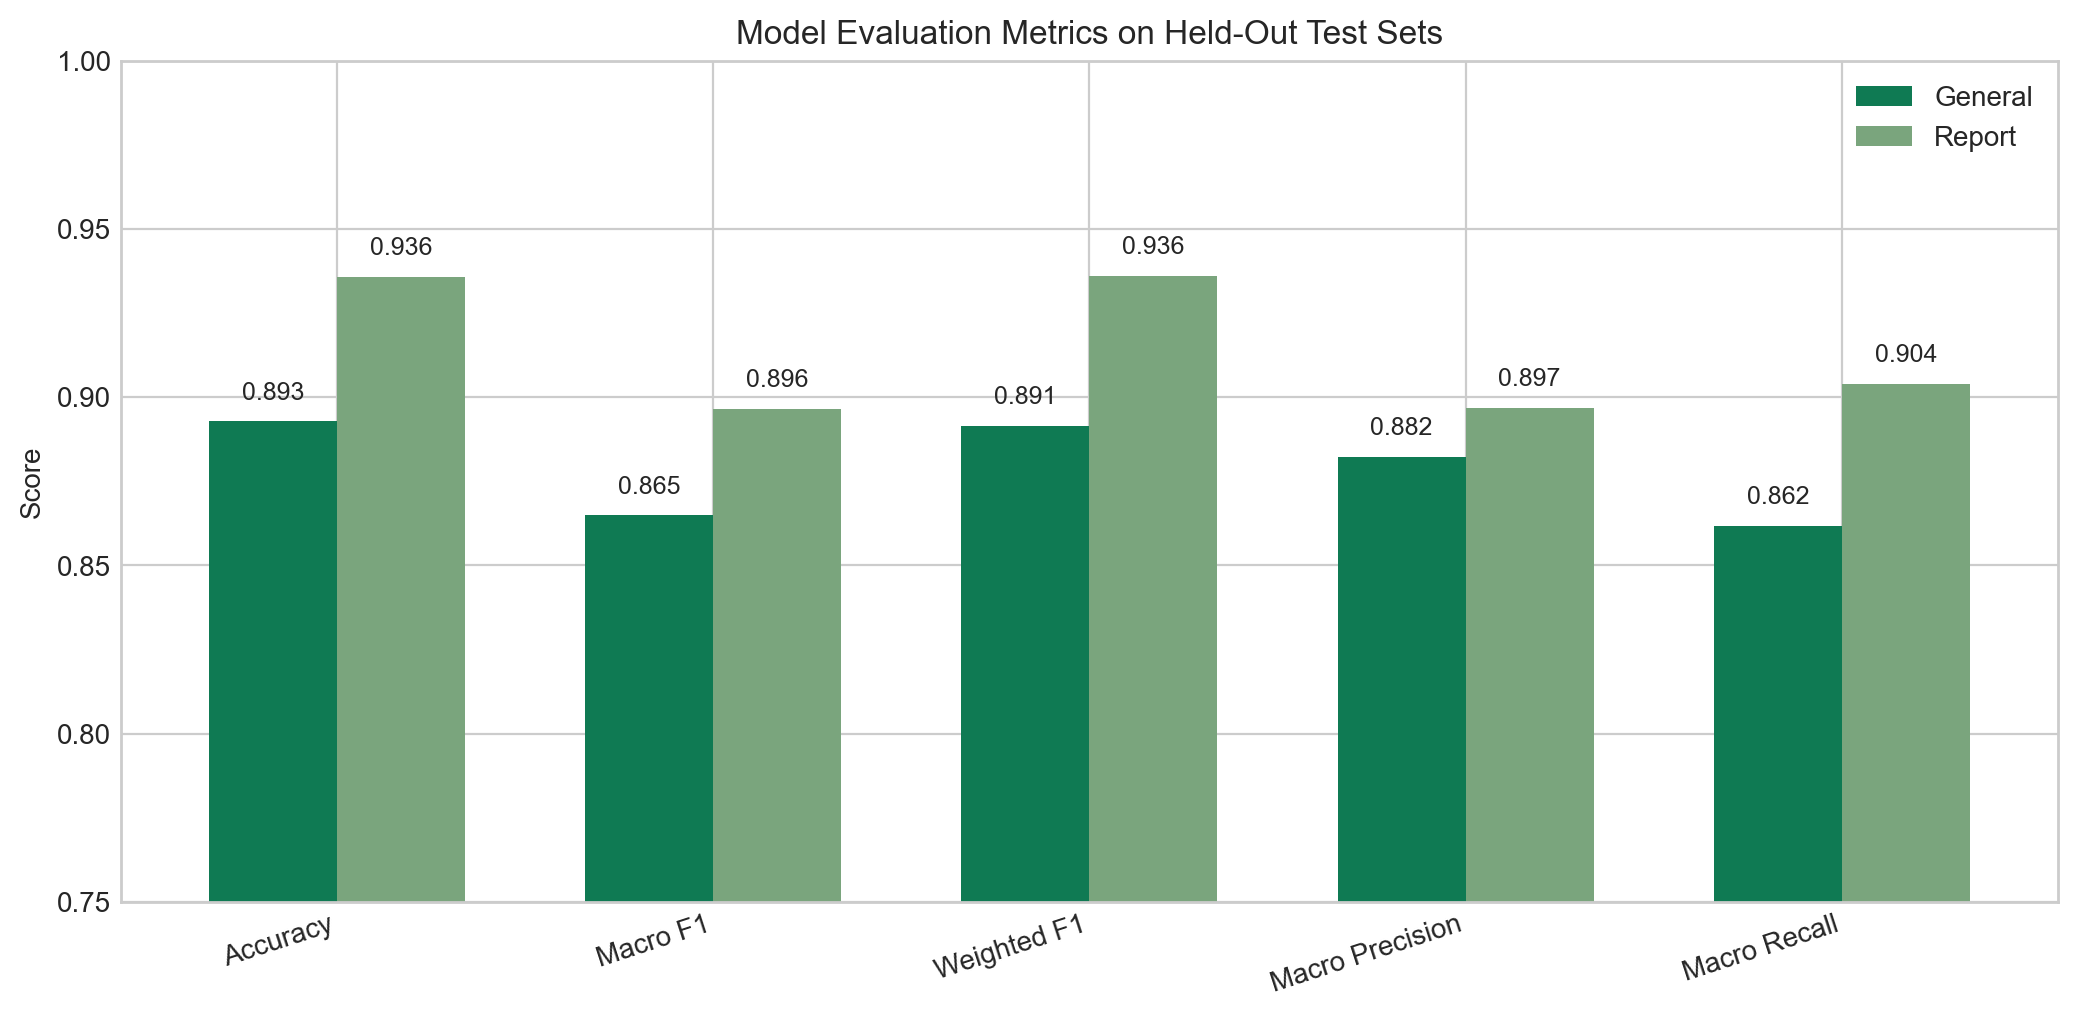
\includegraphics[width=0.88\linewidth]{figures/metric_comparison.png}
    \caption{Metric comparison across the general and report model profiles.}
    \label{fig:metric-comparison}
\end{figure}

\begin{figure}[H]
    \centering
    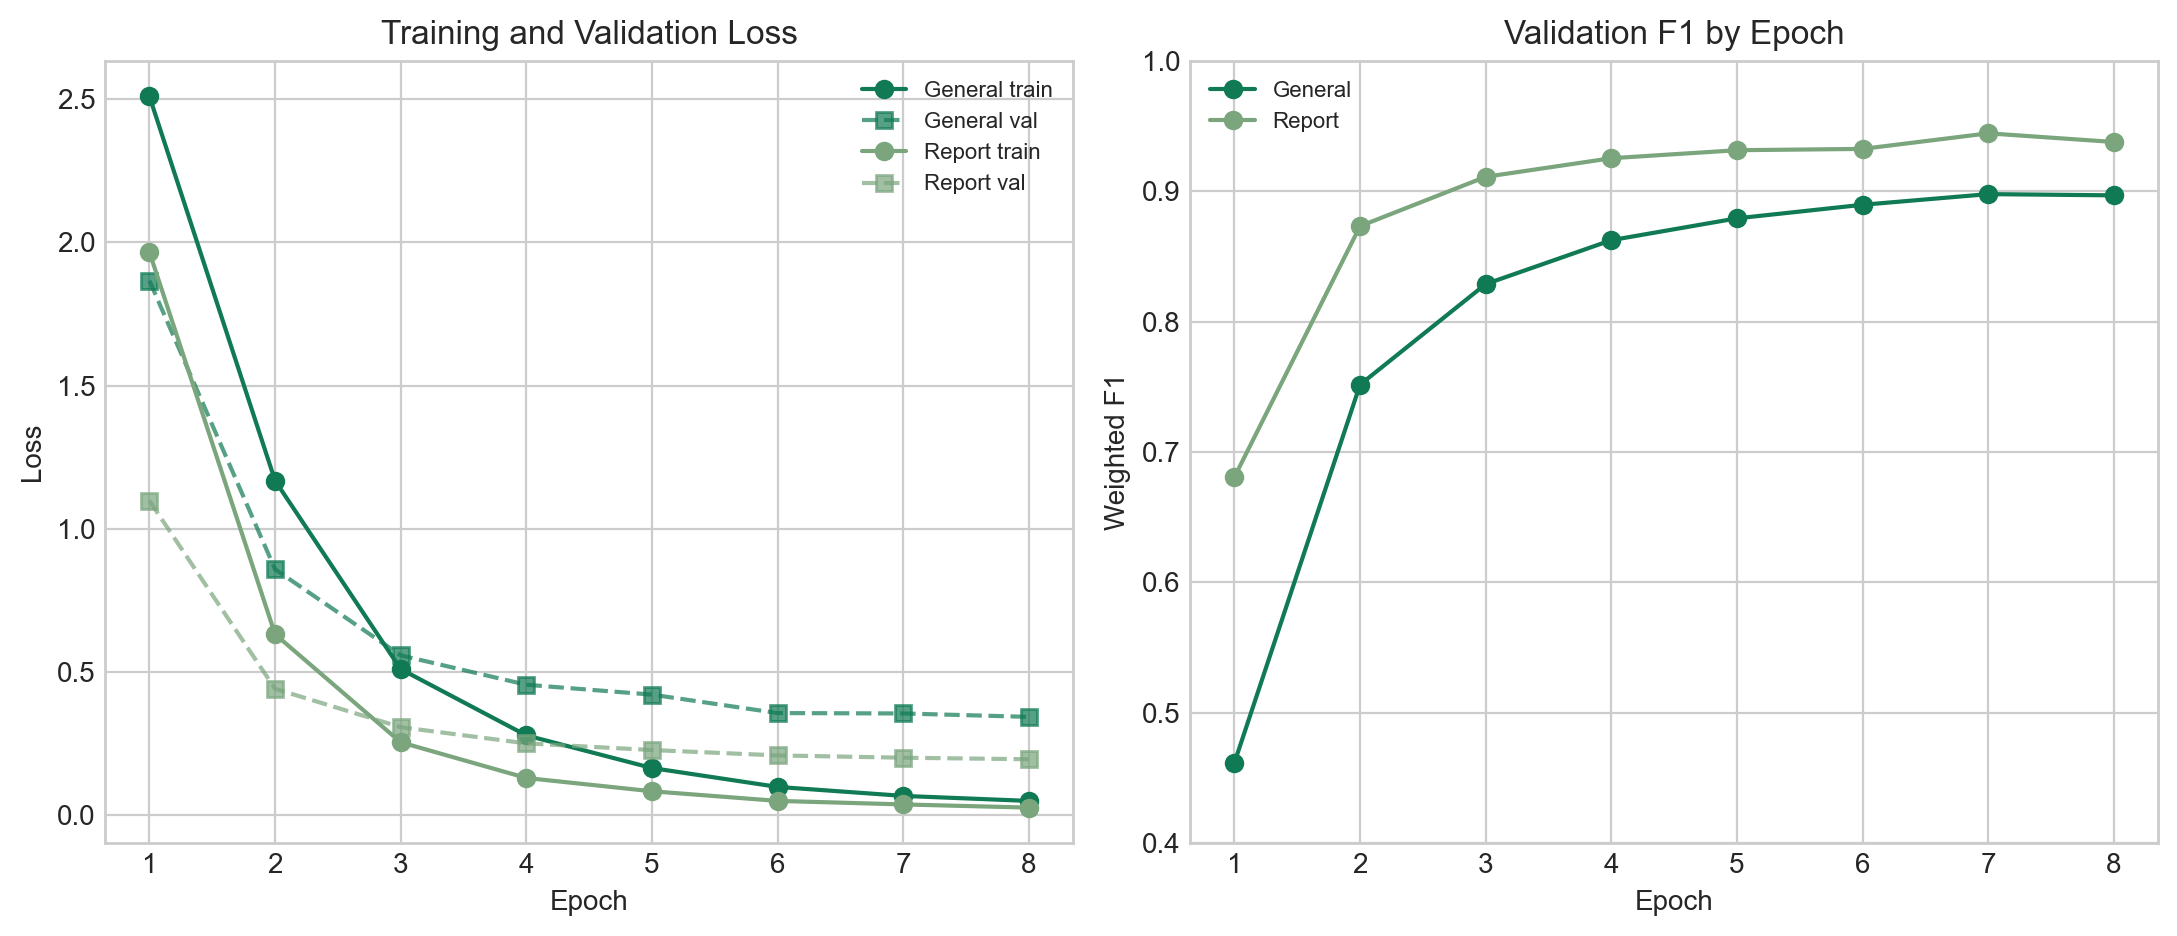
\includegraphics[width=0.88\linewidth]{figures/training_curves.png}
    \caption{Training loss and validation F1 behaviour over the eight-epoch schedule.}
    \label{fig:training-curves}
\end{figure}

\begin{figure}[H]
    \centering
    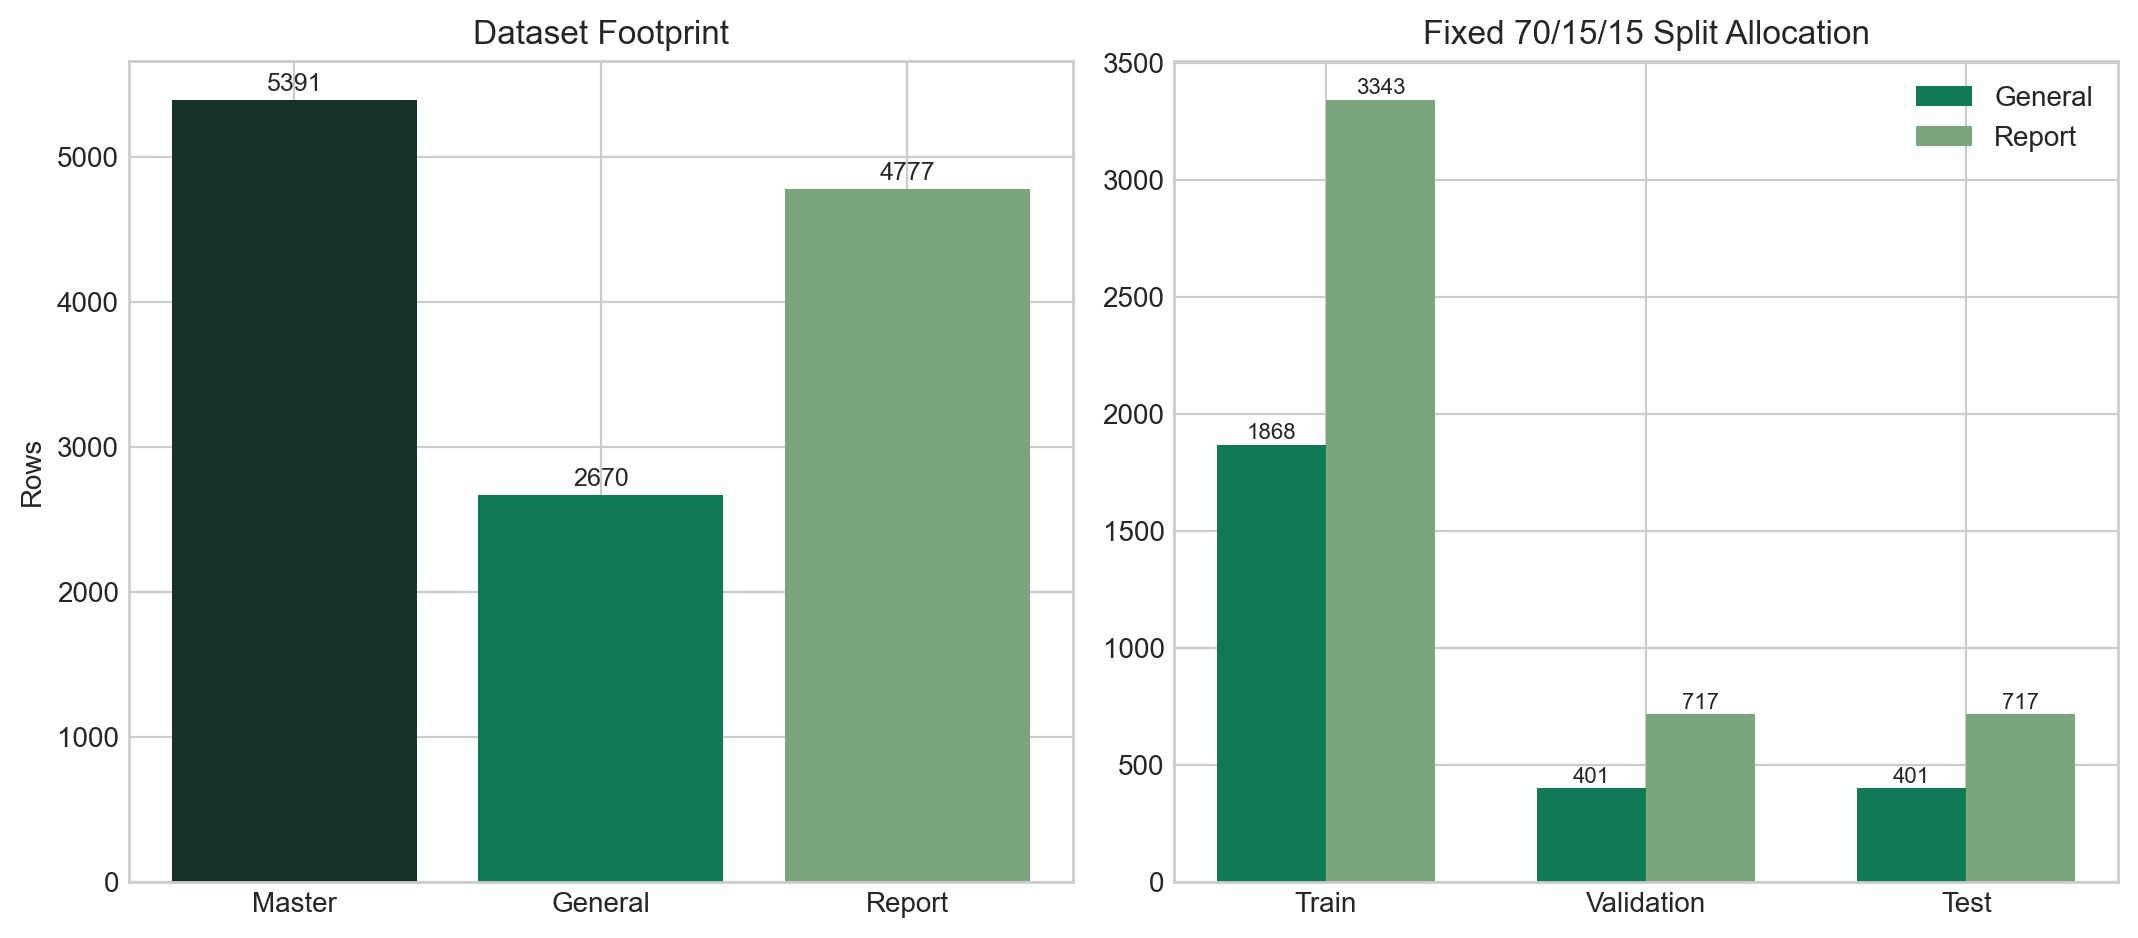
\includegraphics[width=0.88\linewidth]{figures/dataset_splits.png}
    \caption{Dataset footprint and fixed 70/15/15 split allocation.}
    \label{fig:dataset-splits}
\end{figure}

The split-aware evaluation produced more conservative but more defensible results than the earlier single-holdout runs. The general model achieved 0.8928 accuracy, 0.8649 macro F1, 0.8914 weighted F1, 0.8822 macro precision, and 0.8617 macro recall on 401 test examples. The report model achieved 0.9358 accuracy, 0.8965 macro F1, 0.9360 weighted F1, 0.8968 macro precision, and 0.9040 macro recall on 717 test examples after the report-analysis retraining cycle.

These values were strong enough for the scope of the project, especially given the multi-intent label space and safety-oriented conversation classes. The report model achieved higher accuracy after focused data expansion because its report-focused dataset was extended with numeric phrases, printed flags, paediatric phrasing, sex-specific HGB/HCT cases, age-aware prompts, and multi-value report inputs. The general model still faced a broader operational scope, including communication and safety intents, which introduced more heterogeneous phrasing.

\subsection{Training Behaviour, Bias, and Variance Discussion}

The recorded training histories suggested that both models improved steadily over the 8-epoch schedule. For the general model, training loss decreased from 2.5087 to 0.0509 while validation F1 increased from 0.4617 to a best of 0.8978. For the report model, training loss decreased from 1.9654 to 0.0275 while validation F1 increased from 0.6808 to a best of 0.9444. This indicated that the models were not underfitting.

However, the final test macro F1 values of 0.8649 and 0.8965 were lower than the best validation F1 values, which suggested that some generalisation gap remained. That gap was not severe enough to invalidate the models, but it demonstrated that the project could not claim perfect robustness. Several causes were plausible: moderate dataset size, class imbalance, overlap in domain vocabulary, synthetic paraphrase influence, and remaining variation in real conversational phrasing.

It would have been simplistic to describe every output weakness as bias or variance alone. In this project, failure cases also emerged from retrieval coverage gaps, intent overlap, and routing policy. This observation was important because it showed why MLOps evaluation had to go beyond a single classifier score.

\begin{figure}[H]
    \centering
    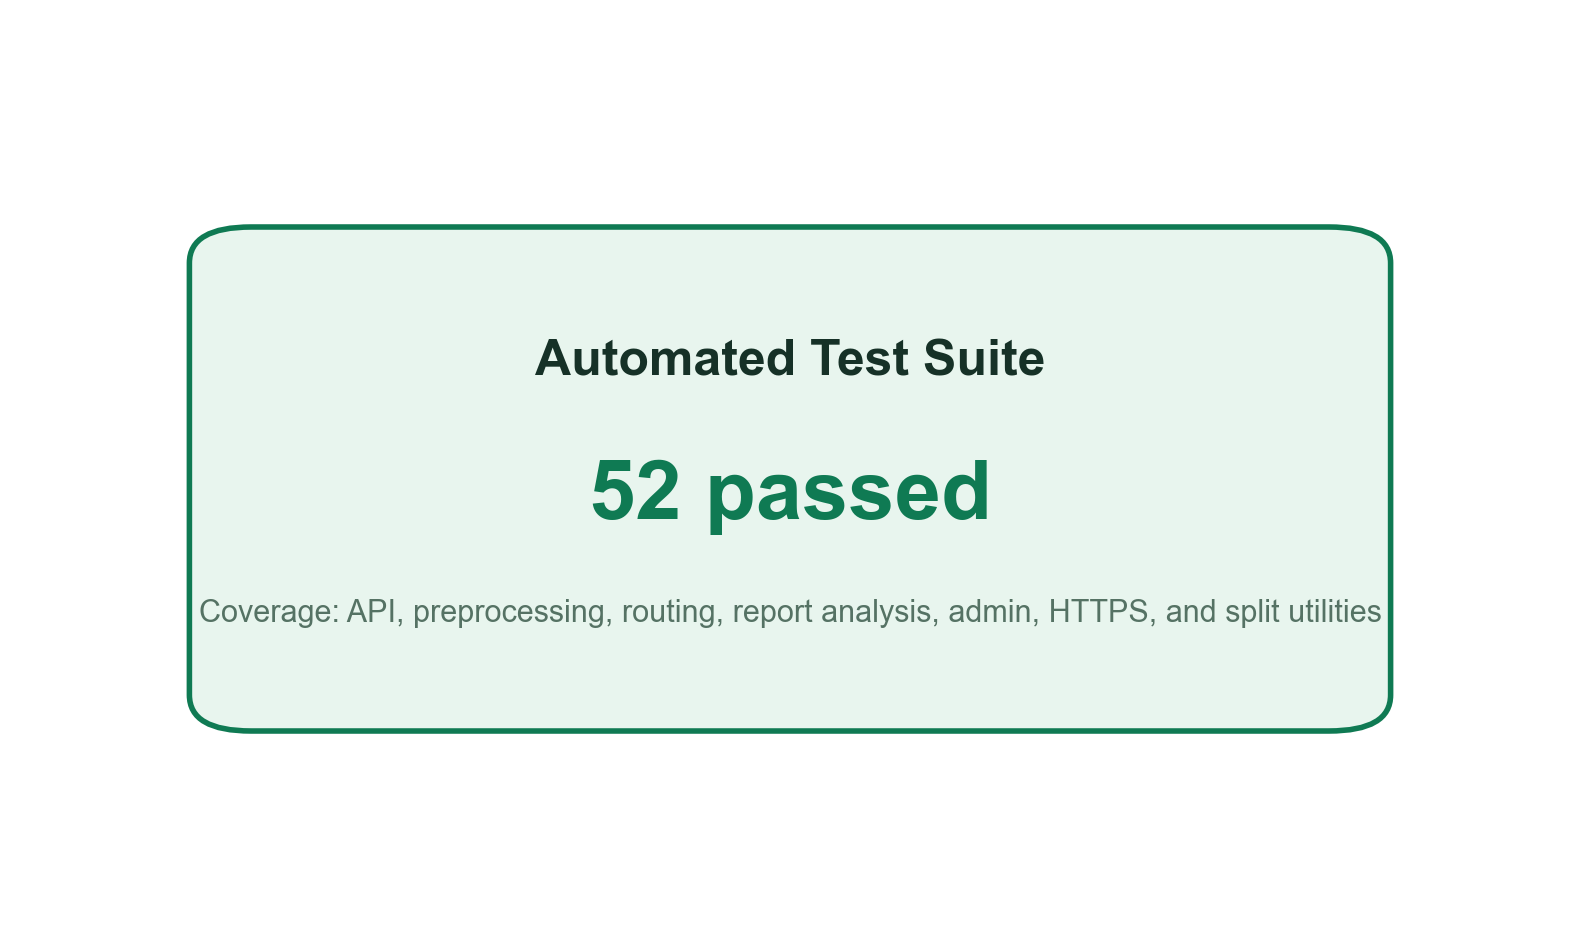
\includegraphics[width=0.72\linewidth]{figures/testing_summary.png}
    \caption{Automated test execution summary showing 52 passing tests.}
    \label{fig:testing-summary}
\end{figure}

At the time of final verification, the full automated test suite passed with 52 tests. These tests covered the major subsystems of the artefact:

\begin{itemize}

\item API endpoint behaviour.

\item Text preprocessing functions.

\item Inference post-processing and fallback handling.

\item Entity detection rules.

\item Routing priorities.

\item Model advisory and auto-switch logic.

\item Predictor rule shortcuts.

\item Report-analysis extraction and interpretation.

\item HTTPS deployment helpers and certificate monitoring.

\item Split generation utilities.

\end{itemize}

This testing strategy aligned with software engineering practice rather than model-only experimentation. It was particularly valuable for regression control. During development, changes to routing and admin features could have introduced silent failures in other areas. The automated suite reduced that risk.

\begin{figure}[H]
    \centering
    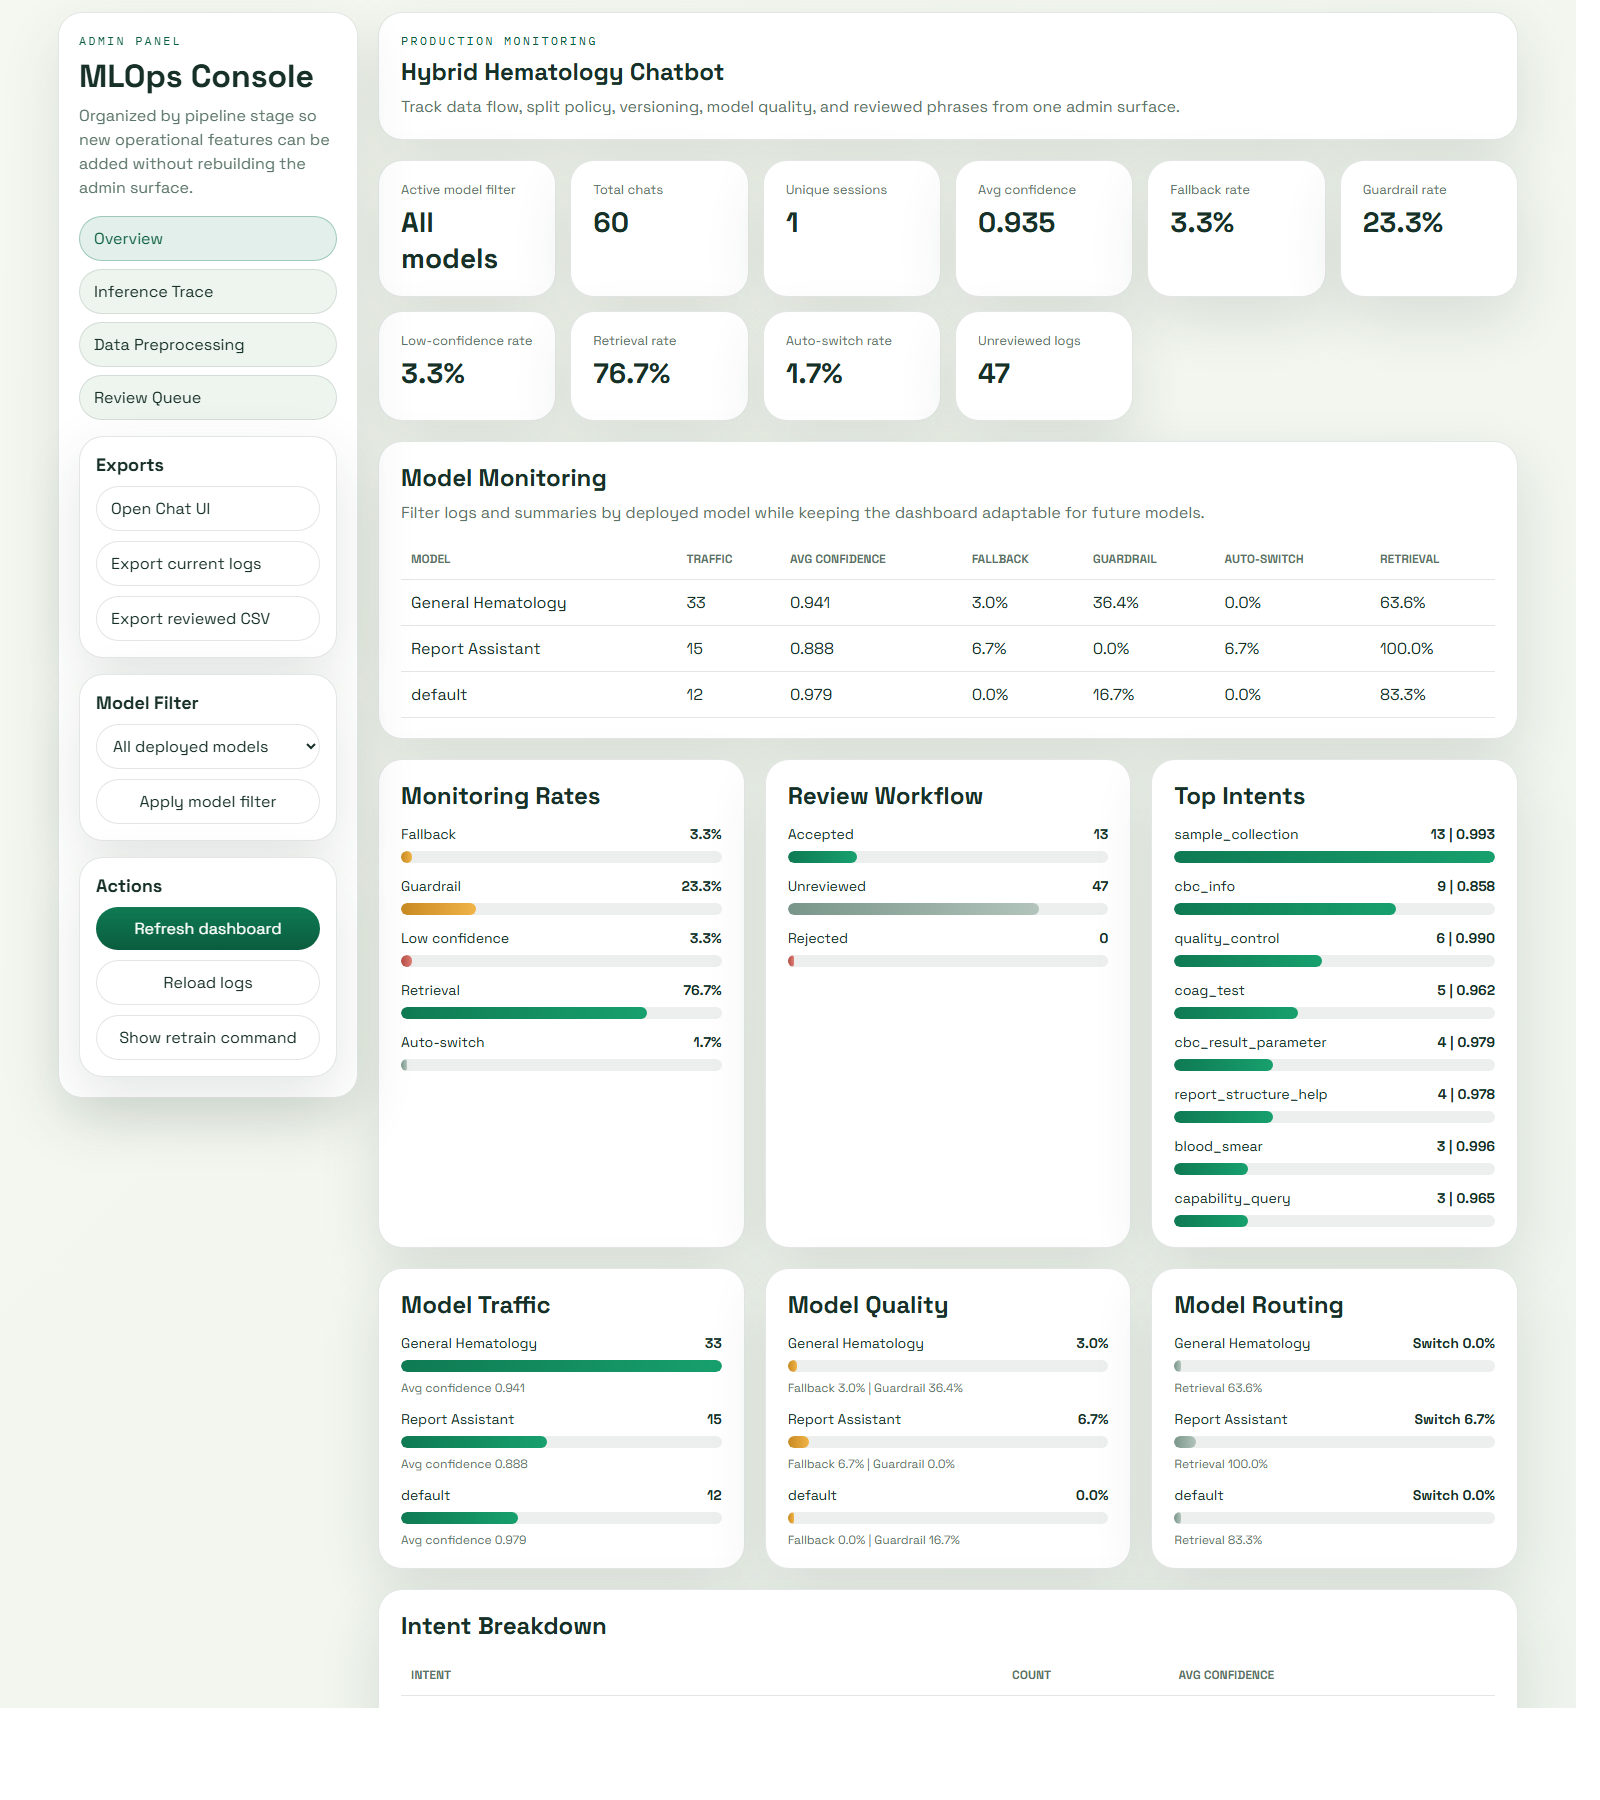
\includegraphics[width=0.88\linewidth]{figures/admin_overview.png}
    \caption{Admin overview dashboard used for operational monitoring and review.}
    \label{fig:admin-overview}
\end{figure}

\begin{figure}[H]
    \centering
    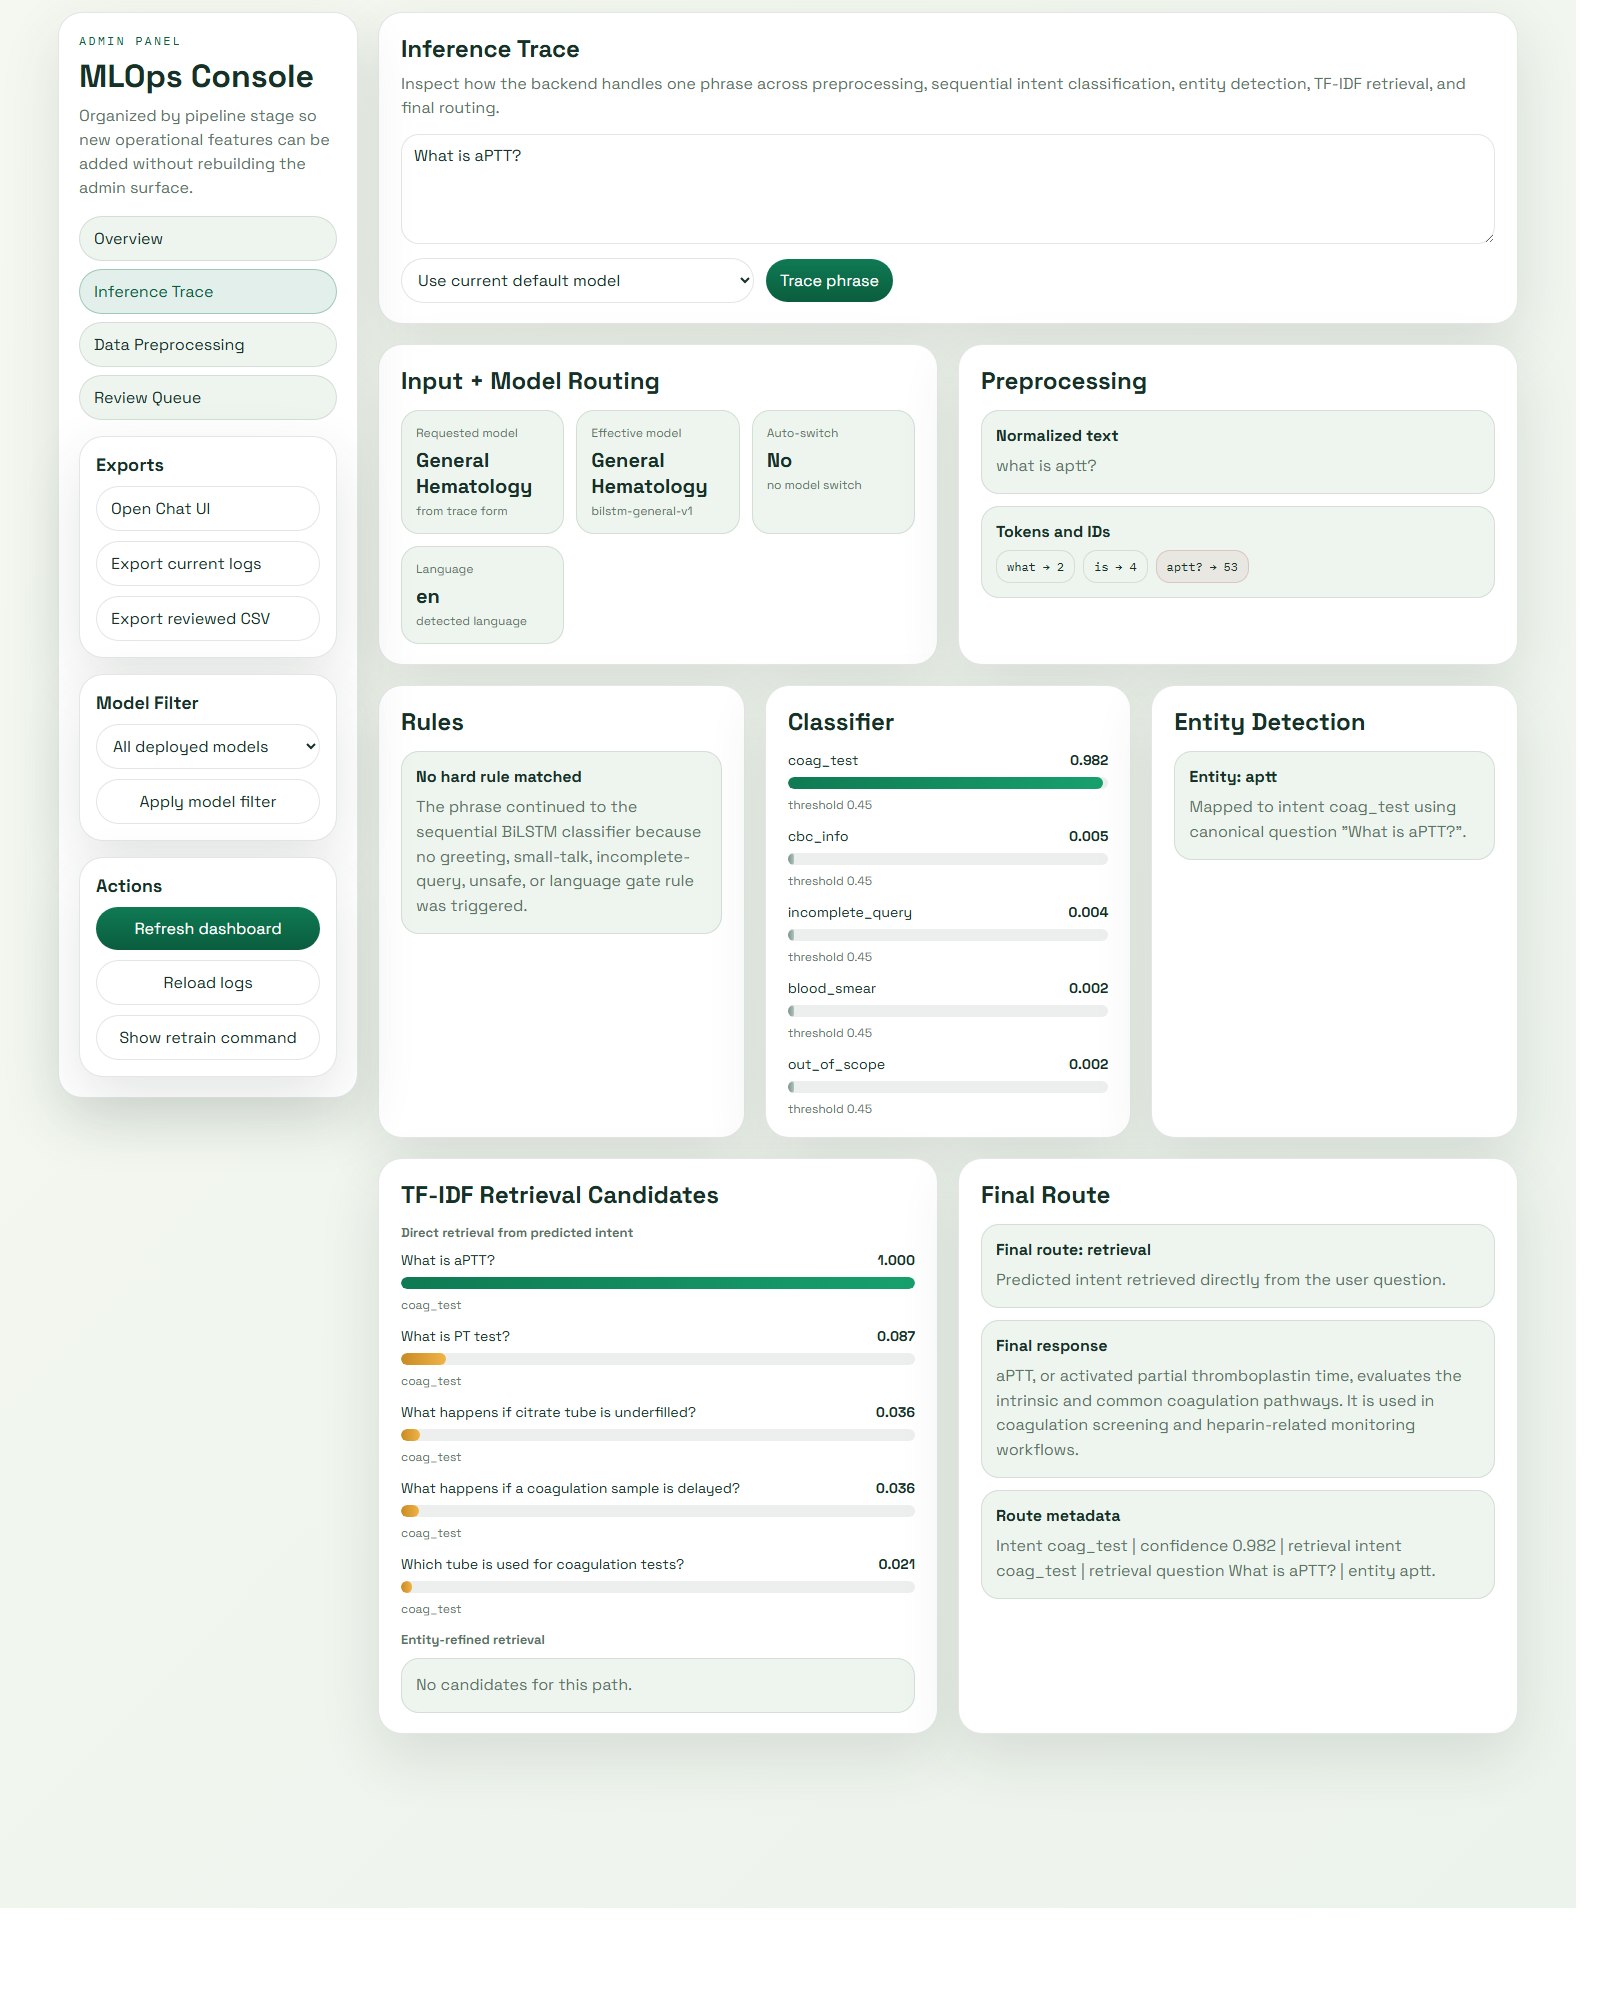
\includegraphics[width=0.88\linewidth]{figures/admin_trace.png}
    \caption{Inference trace view showing how a phrase was processed across the NLP pipeline.}
    \label{fig:admin-trace}
\end{figure}

The admin console provided evidence that the system was not merely trainable but operable. The overview displayed chat volume, average confidence, fallback rate, low-confidence rate, guardrail rate, retrieval rate, and auto-switch rate. The data preprocessing view exposed labelled sources, dataset footprints, version-relevant timestamps, and fixed split counts. The review queue supported log inspection and correction of misclassified phrases. The inference trace exposed how the backend handled an individual question.

The final browser UI also exposed a model-aware coverage panel so that the supported haematology topics of the \texttt{general} and \texttt{report} models were visible to the user. This reduced ambiguity around what each model was expected to do and aligned the interface more closely with the underlying architecture.

From an MLOps perspective, this was a major project strength. The system did not rely solely on offline metrics. Instead, it supported observation of live traffic, review of weak queries, export of reviewed phrases, and retraining from feedback. In practical terms, this meant the system could improve through usage rather than remaining a static demo.

\subsection{Advantages of the Implemented Approach}

Several advantages became clear during evaluation.

First, the sequential BiLSTM design remained computationally lightweight and practical for local deployment. Second, the retrieval-based response layer preserved answer control in a sensitive medical context. Third, the two-model architecture separated workflow support from report support while still allowing automatic switching for convenience. Fourth, the split-aware training and evaluation pipeline improved the credibility of reported metrics. Fifth, the admin console, PostgreSQL logging, and retraining workflow provided a meaningful MLOps foundation rarely present in student chatbot projects.

An additional advantage was interpretability at the system level. Although the BiLSTM itself was still a neural model, the surrounding pipeline made the overall decision process more transparent. Tokenisation, top intent probabilities, entity routing, and retrieval candidates could all be inspected.

\subsection{Limitations}

The project also had clear limitations.

The first limitation was dataset scale. Although 5,391 labelled utterances were substantial for a final-year project, they were still modest compared with industrial NLP datasets. The second limitation was class imbalance. The report dataset imbalance ratio rose because report-analysis phrases became much more common than several smaller support intents. The third limitation was language coverage. Only English was supported. The fourth limitation was that entity detection and report-value extraction remained rule-based, which was efficient and inspectable but not semantically complete. The fifth limitation was scope restriction: the system did not provide diagnosis, treatment recommendations, or unrestricted patient-specific report interpretation.

A further limitation concerned formal user evaluation. While the admin interface and conversation flow were developed carefully, no large-scale human-subject usability study was completed within the project timeline. Therefore, usability claims had to remain cautious and evidence-based rather than overstated.

\subsection{Critical Reflection}

The most important critical lesson was that chatbot quality did not depend solely on the classifier. Several development issues initially appeared to be model failures but were later shown to be retrieval or routing problems. For example, a correctly predicted \texttt{sample\_collection} intent could still return a generic CBC response if broad entity routing was allowed to override operational scope. This reinforced the importance of evaluating the complete pipeline rather than treating the model as the only meaningful component.

A second lesson was that production-style machine learning requires explicit metadata, version awareness, and repeatable data handling. Once fixed splits, review-driven retraining, and monitoring had been added, the project became much stronger academically and technically. Those features did not move the system away from sequential modelling or retrieval-based generation; they made that architecture maintainable.
